\documentclass{anstrans}
\usepackage[acronym,toc]{glossaries}
 \newacronym{iaea}{IAEA}{International Atomic Energy Agency}
 \newacronym{oncore}{ONCORE}{Open-source Nuclear COdes for REactor analysis}
\newacronym{oss}{OSS}{open source software}
\newacronym{rnd}{R\&D}{research and development}
\newacronym{mns}{M\&S}{modelling and simulation}
\newacronym{ent}{E\&T}{education and training}
\newacronym{nrc}{NRC}{Nuclear Regulatory Commission}

%%%%%%%%%%%%%%%%%%%%%%%%%%%%%%%%%%%
\title{Useful practices in open-source software development for nuclear science and engineering}
\author{Oleksandr R Yardas,$^{*}$}

\institute{
$^{*}$Advanced Reactors and Fuel Cycles, University of Illinois - Urbana Champaign.
Champaign, IL, oyardas2@illinois.edu
}

% Optional disclaimer: remove this command to hide
\disclaimer{Notice: this manuscript is a work of fiction. Any resemblance to
actual articles, living or dead, is purely coincidental.}

%%%% packages and definitions (optional)
\usepackage{graphicx} % allows inclusion of graphics
\usepackage{booktabs} % nice rules (thick lines) for tables
\usepackage{microtype} % improves typography for PDF

\newcommand{\SN}{S$_N$}
\renewcommand{\vec}[1]{\bm{#1}} %vector is bold italic
\newcommand{\vd}{\bm{\cdot}} % slightly bold vector dot
\newcommand{\grad}{\vec{\nabla}} % gradient
\newcommand{\ud}{\mathop{}\!\mathrm{d}} % upright derivative symbol

\begin{document}
%%%%%%%%%%%%%%%%%%%%%%%%%%%%%%%%%%%%%%%%%%%%%%%%%%%%%%%%%%%%%%%%%%%%%%%%%%%%%%%%
\section{Introduction (Heading A)}
    Historically, software used in licensing, \Gls{rnd}, and \Gls{ent} efforts in the nuclear field have been closed source and proprietary. (cite) For \Gls{rnd} and \Gls{ent} efforts in particular, this can bring collaborative efforts to a grinding halt until regulatory bodies grant software licences. Using closed codes in scientific publications and research presents barriers to ease of reproducibility and the ability of external verification of results.
    
    Regulatory bodies will require new software features (and in some cases entirely new software tools) in order to effectively and efficiently perform licensing activities for the next generation of advanced reactor designs \cite{usnrc_nonlwr_2020-1}, and many of the open source tools emerging in the past decade (e.g. OpenMC\cite{romano_openmc_2015}) have the advantage over their legacy closed code ancestors (e.g. Serpent \cite{leppanen_serpent_2014}) of using best-practices for software development. It follows that these features and tools are more readily implementable in these new open source projects than in the legacy closed codes.
    
    We are entering the era of \Gls{oss} purpose-built for applications in nuclear science and engineering. This is perhaps best seen in the \Gls{iaea} facilitated \Gls{oncore} initiative \cite{fiorina_initiative_2021} to "[promote] development and application of open- source multi-physics simulation tools to support research, education, and training for analysis of advanced nuclear power reactors"  \cite{iaea_open-source_2022}. Open source development can be complicated and overwhelming with all
    different tasks, checkboxes and rules to follow. There are a few key concepts that developers both new and old should keep in mind in the course of their work. In this abstract, I detail these concepts concepts I have integrated into my own development workflow as part of maintaining and advancing the open source tool Saltproc\cite{rykhlevskii_arfcsaltproc_2018}.

%%%%%%%%%%%%%%%%%%%%%%%%%%%%%%%%%%%%%%%%%%%%%%%%%%%%%%%%%%%%%%%%%%%%%%%%%%%%%%%%
\section{Version control}
    Imagine you are writing a paper for a conference. You spend all day working on the introduction and first few sections, then you accidentally highlight all the text and press the delete key. Luckily you've been using computers for a while, and with a stroke of your fingers\footnote{across the \verb.Ctrl + Z. keys}, all your hard work is saved! In more formal language, when you press \verb.Ctrl + Z., you revert the state of your manuscript to a previous version.
    
    The concept that documents -- or more generally, files -- have a state is the key idea behind {\it version control}. A software project typically has more than one file, and many of these files have states that need to be tracked. Since developers may work on different features in parallel, we'd also like a way to merge multiple changes from different sources into the main software project. Additionally, we should be able to search through the entire history of the project in case we ever need to undo a change or revisit an older version of the software. Version control tools such at \verb.git. and \verb.svn. provide developers a method to work on software with these features in their workflow.
    
    Let's look at a hypothetical scenario. Assume a developer has a feature idea for a software project. Assuming they know how to implement it, how would they use version control in their workflow? The first step in any new feature is to create a {\it branch} -- effectively a copy of the {\it states} of all the files in the project -- in which they will develop their new feature. On the feature branch, our developer writes codes in small steps, adding an annotation for each step. These annotations are called {\it commits}, and are made through the version control tool rather than made in the code itself. Once the developer has finished implementing their feature and has added tests to ensure that the feature is working, they will {\it merge} the feature branch into the main branch. Figure \ref{fig:gh-flow} graphically summarizes this workflow.
    
    \begin{figure}[ht] % replace 't' with 'b' to force it to be on the bottom
      \centering
      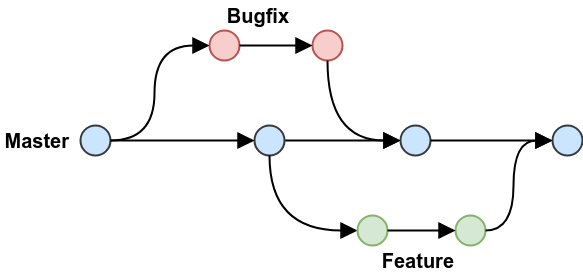
\includegraphics[width=\linewidth]{github-flow.png}
      \caption{Simple branching workflow example \cite{git_flow_fig}}
      \label{fig:gh-flow}
    \end{figure}

%%%%%%%%%%%%%%%%%%%%%%%%%%%%%%%%%%%%%%%%%%%%%%%%%%%%%%%%%%%%%%%%%%%%%%%%%%%%%%%%
\section{Open-development workflow}

    {\it Open development} \footnote{distinct from {\it open-source development} which is closely related but more general}  is a concept in the \Gls{oss} community that emphasizes reproducibility at all scales of the normal development workflow, from individual commits to full releases. In practice, this means more writing for the developer. The benefit is an extremely detailed human readable and searchable record of every decision and change in a piece of software, which is incredibly useful for bringing external and new contributors up to speed. I use an open development workflow in my maintainer role for SaltProc.
    
    Returning to our hypothetical example, let's look at the series of events when the developer has an initial idea for their new feature. Typically, the developer would go to their issue tracker and make a new issue that is a very basic summary of their idea. In an open development model, the developer needs to describe the background and motivation for the feature, describe the feature itself, provide specific implementation details and useful resources for the feature, and list any potential snags that could come up while implementing the feature. In essence, the developer needs to think and come up with a plan for their feature before they even start writing any code\footnote{A good real-world example of this is issue \#109 in the SaltProc repository (https://github.com/arfc/saltproc/109)}.
    
    Using open development in your workflow guarantees that other developers will know the purpose or context for a new feature.
    
%%%%%%%%%%%%%%%%%%%%%%%%%%%%%%%%%%%%%%%%%%%%%%%%%%%%%%%%%%%%%%%%%%%%%%%%%%%%%%%%
\section{Automation and continuous integration}
    Many of the tasks developers spend time on are menial and repetitive. Examples of such tasks include running test suites, building documentation, assigning labels in issue trackers, creating new release notes, and so on. These tasks, while important, require time and attention that developers could be using on designing improvements and features to the code. The repetitive, template-like nature of these tasks make them well suited to {\it automation}. Automation, as the name implies, refers to the process of automatically carrying out a set of user-defined tasks based on some condition. Given sufficient knowledge of an operating system, a user could implement their own methods for creating and running automated tasks. In practice, services like GitHub Actions and CircleCI provide a framework for developers to easily add automation into their development workflow. These services depend on user-created instruction sets -- called {\it workflows} -- that execute when certain events happen.

     I have created two particularly useful workflows in the course of maintaining SaltProc that do the following:
     \begin{itemize}
         \item deploys web-hosted documentation when there is a change in the source code or doc pages
         \item populate release notes to multiple locations in different formats when a release is published
         \item update the software version specified in the configuration files when a release is published
     \end{itemize}
     While these tasks are not difficult to do manually, they are time consuming and automating them leaves more space for me to add features, implement bug fixes, and interact with my users.
    
    Going back to our hypothetical example, let's assume that the developer has implemented the feature in the source code and added tests for that feature. They commit it to their development branch, but before merging the feature into the main branch, they need to run the tests to make sure the code still works as intended. With automation, as soon as that commit is made, the test suite runs on the updated code. This is known as {\it continuous integration} (CI). CI enables quick detection of bugs an implementation errors. CI also makes sure that tests pass before merging a feature into the main branch, avoiding the potential hassle of reverting a merge.
    

\section{Conclusions (Heading A)}



%%%%%%%%%%%%%%%%%%%%%%%%%%%%%%%%%%%%%%%%%%%%%%%%%%%%%%%%%%%%%%%%%%%%%%%%%%%%%%%%
\section{Acknowledgments}
This work is supported by the NRC Integrated University Grant Program Fellowship.

%%%%%%%%%%%%%%%%%%%%%%%%%%%%%%%%%%%%%%%%%%%%%%%%%%%%%%%%%%%%%%%%%%%%%%%%%%%%%%%%
\bibliographystyle{ans}
\bibliography{bibliography}
\end{document}

